

\documentclass[12pt,english,titlepage]{article}
\usepackage{Ecology}
\title{Long Title}
\author[1]{Author, First}
\author[2]{Author, Second}
\affil[1]{Dept. of , X University, 100 College Way, College Town 10001}
\affil[2]{Dept. of , Y University, 200 University Lane, Big City 99999}

\date{} % Activate to display a given date or no date (if empty),
         % otherwise the current date is printed 
\runninghead{Short Title}
\begin{document}
\maketitle
\begin{spacing}{1.9}
\begin{abstract}
This is the abstact
\end{abstract}

\keywords{List; of ; Keywords; Here}
\begin{flushleft}
\section{Introduction}

\section{Methods}

\subsection{Subsection}

\section{Results}

\section{Discussion} 

\section{Conclusion}

\section*{Acknowledgements}

\section{Literature Cited}

LastName, F.A. and S.A. LastName. YYYY.  Title. \textit{Journal} \textbf{1}:xx-xx.\\

\newpage
\section{Tables}
Table 1. Stuff here

\begin{tabular}{l|c|c|c|c}
              & A & B &C & D \\    
\hline
$a$ &142.67& 23.97 &  5.95 & $<.0.01$ \\
$b$   &  209.65 & 25.75  & 2.60  & $<.0.01$  \\
$c$   &362.88  & 26.53  & 8.30 & $<.0.01$ \\

\end{tabular}
\vskip 1cm
\newpage

\section{Figure Legends}

Figure 1 -- Figure Legend\\
\vspace{5mm}

\newpage

\section{Figures}

\begin{figure}[!h]
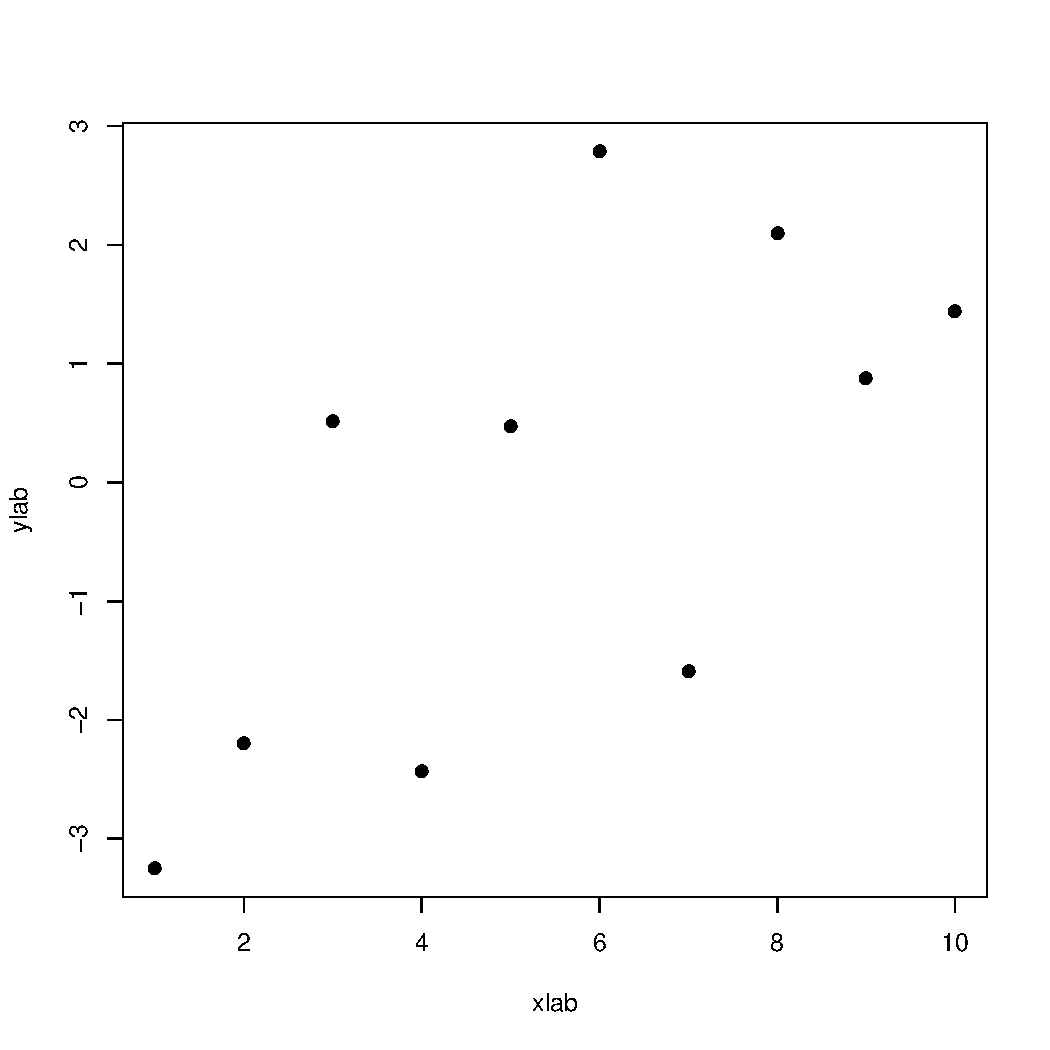
\includegraphics[width=\textwidth]{graph.pdf}
\caption{}
\end{figure}
\newpage


\end{flushleft}
\end{spacing}
\end{document}
